\documentclass[tikz]{standalone}
\usepackage{tikz}
\usetikzlibrary{shadings,positioning,shadows.blur,backgrounds,calc,math}
\usepackage{xcolor}

\newlength\longd
\newlength\shortd
\setlength{\longd}{0.5cm}
\setlength{\shortd}{0.2cm}
\newcommand{\islamicshape}[3]{
   \shadedraw[inner color=#1,outer color=#2, draw=#3 ]
   (O)[rounded corners=4pt] --
   ++(90:\longd)[sharp corners] --
   ++(210:\shortd)[rounded corners=4pt] --
   ++(150:\shortd) --
   ++(30:\longd)--
   ++(330:\longd)[sharp corners] --
   ++(210:\shortd)[rounded corners=4pt] --
   ++(150:\shortd)--
   ++(-90:\longd) --
   ++(90-120:\longd) [sharp corners]--
   ++(210-120:\shortd)[rounded corners=4pt] --
   ++(150-120:\shortd)--
   ++(30-120:\longd) --
   ++(330-120:\longd)[sharp corners] --
   ++(210-120:\shortd)[rounded corners=4pt]--
   ++(150-120:\shortd)--
   ++(-90-120:\longd) --
   ++(90-240:\longd) [sharp corners]--
   ++(210-240:\shortd)[rounded corners=4pt] --
   ++(150-240:\shortd) --
   ++(30-240:\longd) --
   ++(330-240:\longd)[sharp corners] --
   ++(210-240:\shortd)[rounded corners=4pt] --
   ++(150-240:\shortd)-- cycle;
}
\def\thisshape{\islamicshape}

\begin{document}
\pagecolor{transparent}
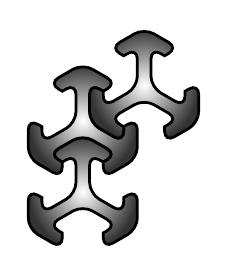
\begin{tikzpicture}[transparency group=knockout]
    \coordinate (O) at (0,0);
    %\thisshape{black!80}{white}{white};
    \thisshape{white}{black!80}{black!240};
    \coordinate (O) at (0,4.5*\shortd);
    \thisshape{white}{black!80}{black!240};
    \coordinate (O) at (${0.5*sqrt(3)*4.5}*(\shortd,0)+(0,6.75*\shortd)$);
    \thisshape{white}{black!80}{black!240};
\end{tikzpicture}
\end{document}